\section{解的性质}
\label{sec:opt-properties}

知道解存在之后，自然要问这个解是什么样的：洼地的底部是不是最低处？最低点是不是只有一个？目标值接近最优时，位置也接近吗？这些问题都在比较两个候选，最简单的比较路径是连接它们的线段。本节一路沿线段比较，逐步加强要求，依次回答这三个问题。

\paragraph{凸集：线段留在里面}
资源分配中，方案$\bm{u}=(3,0)$与$\bm{v}=(0,4)$都可行。各执行一半，得到混合方案$\frac12\bm{u}+\frac12\bm{v}=(1.5,2)$，它也可行，因为$1.5+2=3.5\leq4$，$3+2=5\leq6$，产量也非负。

这不是巧合。若$\bm{u},\bm{v}$都满足同一个线性不等式$\langle\bm{a},\bm{x}\rangle\leq c$，则对$\theta\in[0,1]$，
\[
 \langle\bm{a},\theta\bm{u}+(1-\theta)\bm{v}\rangle
 =\theta\langle\bm{a},\bm{u}\rangle+(1-\theta)\langle\bm{a},\bm{v}\rangle
 \leq\theta c+(1-\theta)c=c.
\]
可行方案任意混合仍然可行，这个性质值得单独命名。

\begin{definition}[凸集]
\label{def:opt-convex-set}
若对任意$\bm{u},\bm{v}\in\bm{C}$与$\theta\in[0,1]$，都有
\begin{equation}
 \theta\bm{u}+(1-\theta)\bm{v}\in\bm{C},
 \label{eq:opt-convex-set}
\end{equation}
就称$\bm{C}\subseteq\mathbb{R}^n$为\term{凸集}（convex set）。
\end{definition}

几何上，凸集里任意两点之间的线段都留在集合内。上面的计算说明半空间$\{\bm{x}:\langle\bm{a},\bm{x}\rangle\leq c\}$是凸集。若干凸集的交仍是凸集：两点同时在每个集合中，线段也同时在每个集合中。资源分配的可行集是四个半空间的交，所以是凸集。图~\ref{fig:opt-convex-sets}给出对照。

\begin{BookInlineFigure}
  \centering
  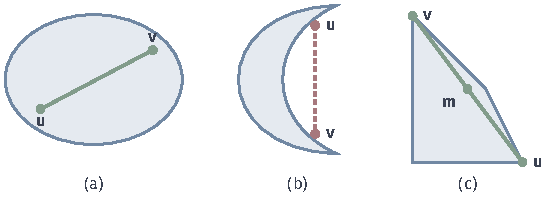
\includegraphics[width=93.691mm]{figures/05-optimization/01-linear-programming/tikz/opt-convex-sets/figure.pdf}
  \caption{凸集与非凸集。(a)椭圆盘中任意两点间的绿色线段留在集合内。(b)月牙形中两点都在集合里，红色虚线却穿过缺口，所以不是凸集。(c)资源分配的可行四边形，$\bm{u}=(3,0)$与$\bm{v}=(0,4)$的等权混合$\bm{m}=(1.5,2)$仍在集合内。}
  \label{fig:opt-convex-sets}
\end{BookInlineFigure}

\paragraph{凸函数：图像不鼓过弦}
可行集凸时，两个可行点之间的线段全是候选。接下来要求目标沿这条线段“不鼓起来”：线段上每一点的目标值，不超过两端目标值按相同权重的平均。

\begin{definition}[凸函数]
\label{def:opt-convex-function}
设$\bm{C}$为凸集。若$f:\bm{C}\to\mathbb{R}$对任意$\bm{u},\bm{v}\in\bm{C}$与$\theta\in[0,1]$满足
\begin{equation}
 f\bigl(\theta\bm{u}+(1-\theta)\bm{v}\bigr)\leq\theta f(\bm{u})+(1-\theta)f(\bm{v}),
 \label{eq:opt-convex-function}
\end{equation}
就称$f$为$\bm{C}$上的\term{凸函数}（convex function）。扩展实值函数称为凸函数，是指其有效定义域为凸集，且式~\eqref{eq:opt-convex-function}对有效定义域中的点成立。
\end{definition}

式~\eqref{eq:opt-convex-function}右端是连接两点$(\bm{u},f(\bm{u}))$与$(\bm{v},f(\bm{v}))$的弦上的点，左端是同一位置的函数值。所以凸函数的图像位于每条弦的下方，也就是碗的形状。图~\ref{fig:opt-chord}(a)是凸函数$x^2/2$；(b)中的函数有两个碗，连接两侧的弦从中间的鼓包下面穿过，不等式被破坏。对$F=f+\iota_{\bm{C}}$，这个定义恰好要求$\bm{C}$凸且$f$在$\bm{C}$上凸。

\begin{BookInlineFigure}
  \centering
  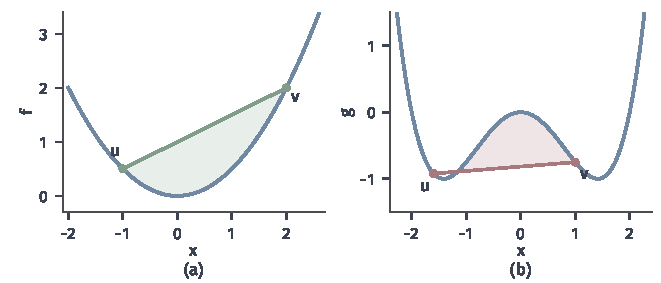
\includegraphics[width=112mm]{figures/05-optimization/01-linear-programming/matplotlib/opt-chord/figure.pdf}
  \caption{图像与弦。(a)凸函数$f(x)=x^2/2$，连接$x=-1$与$x=2$的绿色弦位于图像上方，浅绿区域是两者的间隔。(b)非凸函数$g(x)=x^4/4-x^2$，连接$x=-1.6$与$x=1$的红色弦有一段位于图像下方，浅红区域就是违反凸性的部分。}
  \label{fig:opt-chord}
\end{BookInlineFigure}

二次函数的情形可以算到底。设$\bm{H}\in\mathbb{R}^{n\times n}$对称，考虑
\[
 q(\bm{x})=\frac12\bm{x}^\top\bm{H}\bm{x}+\bm{a}^\top\bm{x}+a_0.
\]
记$\bm{w}=\theta\bm{u}+(1-\theta)\bm{v}$，我们计算弦与函数之间的间隔。线性项和常数项在加权平均中抵消，只需展开二次项：
\[
 \bm{w}^\top\bm{H}\bm{w}=\theta^2\bm{u}^\top\bm{H}\bm{u}+2\theta(1-\theta)\bm{u}^\top\bm{H}\bm{v}+(1-\theta)^2\bm{v}^\top\bm{H}\bm{v}.
\]

用$\theta-\theta^2=\theta(1-\theta)$，以及$(1-\theta)-(1-\theta)^2=\theta(1-\theta)$，得到
\begin{equation}
 \theta q(\bm{u})+(1-\theta)q(\bm{v})-q(\bm{w})=\frac12\theta(1-\theta)(\bm{u}-\bm{v})^\top\bm{H}(\bm{u}-\bm{v}).
 \label{eq:opt-quadratic-gap}
\end{equation}
所以$q$凸当且仅当$\bm{H}$半正定。

二次拟合目标~\eqref{eq:opt-ridge}展开后正是这种形式，其中$\bm{H}=\bm{A}^\top\bm{A}+\gamma\bm{I}$。对任意$\bm{w}$，
\[
 \bm{w}^\top\bm{H}\bm{w}=\lVert\bm{A}\bm{w}\rVert_2^2+\gamma\lVert\bm{w}\rVert_2^2\geq0,
\]
所以目标是凸函数。资源分配的目标是线性函数，式~\eqref{eq:opt-convex-function}取等号，也是凸函数。

\paragraph{局部最优就是全局最优}
现在回答第一个问题：山那边会不会有更深的谷。若目标和可行集都是凸的，答案是不会。

\begin{theorem}[凸问题的局部最优是全局最优]
\label{thm:opt-local-global}
设$\bm{C}$为凸集，$f:\bm{C}\to\mathbb{R}$为凸函数。则$f$在$\bm{C}$上的每个局部最优解都是全局最优解，并且最优解集合是凸集。
\end{theorem}

\begin{proof}
设$\bm{u}$是局部最优解，对应的邻域半径为$r$。假设存在$\bm{v}\in\bm{C}$使$f(\bm{v})<f(\bm{u})$。对$t\in(0,1)$，点$\bm{u}+t(\bm{v}-\bm{u})$在线段上，所以属于$\bm{C}$。由式~\eqref{eq:opt-convex-function}，
\[
 f\bigl(\bm{u}+t(\bm{v}-\bm{u})\bigr)\leq(1-t)f(\bm{u})+tf(\bm{v})<f(\bm{u}).
\]

取$t$足够小，使$t\lVert\bm{v}-\bm{u}\rVert_2<r$，这个更低的点就落在$\bm{C}\cap\bm{B}(\bm{u},r)$中，与局部最优矛盾。所以$\bm{u}$是全局最优解。

若$\bm{u},\bm{v}$都是最优解，线段上的点满足$f\leq\theta f^\star+(1-\theta)f^\star=f^\star$，也是最优解，所以最优解集合是凸集。
\end{proof}

证明的几何意义是：如果远处有更低的点，连向它的弦从当前点一出发就下降，凸函数的图像又在弦下方，紧贴当前点就有更低的点。图~\ref{fig:opt-local-implies-global}用非凸的例子~\ref{ex:opt-local-global}反过来看这件事：局部最优点$u$与更低的点$v$之间，弦在$u$的邻域里就低于$f(u)$，而图像却在弦上方，浅红区域正是对凸性的违反。

\begin{BookInlineFigure}
  \centering
  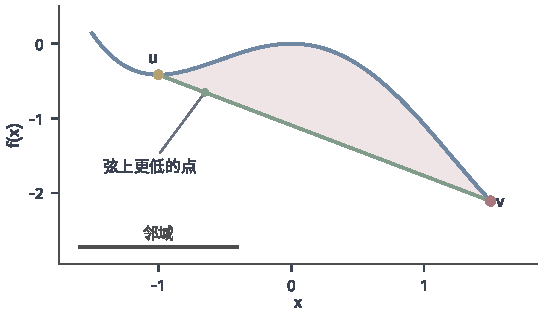
\includegraphics[width=92mm]{figures/05-optimization/01-linear-programming/matplotlib/opt-local-implies-global/figure.pdf}
  \caption{为什么凸问题没有假谷底。蓝线是$f(x)=x^4/4-x^3/3-x^2$，黄点$u=-1$是局部最优解，红点$v=1.5$更低。绿色弦上紧靠$u$的点已经低于$f(u)$，深灰线段是$u$的邻域。若$f$是凸函数，图像就必须在弦下方，$u$的邻域里就有更低的点；浅红区域表明这里的$f$不是凸函数，$u$才得以成为局部最优。}
  \label{fig:opt-local-implies-global}
\end{BookInlineFigure}

可行集和目标两个条件都要有。可行集不凸时，线段会跑出去：在$C=[-3,-1]\cup[1,3]$上最小化凸函数$(x-2)^2$，$x=-1$处的值是$9$，它的邻域里的可行点都在$[-3,-1]$中，函数值都不低于$9$，所以它是局部最优解；全局最优解却是$x=2$，值为$0$。目标不凸时，例子~\ref{ex:opt-local-global}已经给出反例。

\paragraph{严格凸与唯一性}
凸性排除了假谷底，但没有排除平坦的谷底：$\gamma=0$的拟合实例沿直线$x_1+x_2=2$处处最优。资源分配如果把利润改成$2x_1+2x_2$，利润线就与边$x_1+x_2=4$平行，从$(0,4)$到$(2,2)$的整条线段都最优。要让解唯一，需要弦和图像之间确实有间隔。

\begin{definition}[严格凸函数]
\label{def:opt-strict-convex}
设$\bm{C}$为凸集。若$f:\bm{C}\to\mathbb{R}$对任意$\bm{u}\neq\bm{v}$与$\theta\in(0,1)$都使式~\eqref{eq:opt-convex-function}严格成立，就称$f$为\term{严格凸函数}（strictly convex function）。
\end{definition}

\begin{theorem}[严格凸目标至多有一个最小点]
\label{thm:opt-strict-unique}
设$\bm{C}$为凸集，$f$在$\bm{C}$上严格凸，则最优解至多有一个。若最优解存在，则它唯一。
\end{theorem}

\begin{proof}
假设$\bm{u}\neq\bm{v}$都是最优解。中点$\frac12(\bm{u}+\bm{v})\in\bm{C}$，由严格凸性，
\[
 f\Bigl(\frac12(\bm{u}+\bm{v})\Bigr)<\frac12f^\star+\frac12f^\star=f^\star.
\]
这与$f^\star$是下确界矛盾。
\end{proof}

结论是“至多一个”，存在性要由上一节另外保证。正反两个方向都有反例。$e^x$严格凸，却没有最小点，所以严格凸不推出存在。$\lvert x\rvert$有唯一最小点$0$，但在$[0,1]$上是线性的，式~\eqref{eq:opt-convex-function}取等号，不严格凸，所以最小点唯一也不推出严格凸。资源分配更典型：线性目标毫无弯曲，解$(2,2)$仍然唯一，唯一性来自可行集的顶点。

二次函数的严格凸性由式~\eqref{eq:opt-quadratic-gap}直接读出：$\bm{u}\neq\bm{v}$时间隔为正，当且仅当$\bm{H}$正定。若$\bm{H}$半正定但奇异，沿零空间方向的线段上间隔为零。对二次拟合，前面算出的二次型表明，$\gamma>0$或$\bm{A}$列满秩时目标严格凸。

在实例~\eqref{eq:opt-ridge-instance}中，二次型矩阵是
\[
 \bm{H}=\begin{bmatrix}1+\gamma&1\\1&1+\gamma\end{bmatrix}.
\]
$\gamma=0$时$\bm{w}=(1,-1)$使$\bm{w}^\top\bm{H}\bm{w}=0$，解成一条线。

$\gamma>0$时，唯一的解可以手算。记$s=x_1+x_2$，由$x_1^2+x_2^2\geq s^2/2$（等号当且仅当$x_1=x_2$），得到
\[
 f(\bm{x})\geq\frac12(s-2)^2+\frac{\gamma}{4}s^2.
\]
右端是$s$的一元二次函数，令导数$(s-2)+\gamma s/2$为零，得$s=4/(2+\gamma)$。再取$x_1=x_2=s/2$使等号成立，于是
\begin{equation}
 \bm{x}^\star=\frac{2}{2+\gamma}(1,1),\qquad f^\star=\frac{2\gamma}{2+\gamma}.
 \label{eq:opt-ridge-solution}
\end{equation}
例如$\gamma=0.5$时，$\bm{x}^\star=(0.8,0.8)$，$f^\star=0.4$，这正是图~\ref{fig:opt-coercive-sublevel}(b)中的红点。

\paragraph{强凸：间隔有多大}
严格凸只说间隔为正，没说间隔有多大。取$f(x)=x^4$，端点$u=-t$，$v=t$，权重$\theta=\frac12$，弦中点的高度是$t^4$，函数值是$0$，所以间隔只有$t^4$。而两点距离的平方是$4t^2$。$t$很小时，$t^4$比$4t^2$小得多。

间隔太小的后果是：目标值几乎相同的两个点可能相距很远，我们就无法从“目标值差不多最优”推断“位置差不多正确”。强凸性要求间隔至少与距离的平方成比例。

\begin{definition}[强凸函数]
\label{def:opt-strong-convex}
设$\bm{C}$为凸集，$\mu>0$。若对任意$\bm{u},\bm{v}\in\bm{C}$与$\theta\in[0,1]$，
\begin{equation}
 \begin{aligned}
 f\bigl(\theta\bm{u}+(1-\theta)\bm{v}\bigr)\leq{}&\theta f(\bm{u})+(1-\theta)f(\bm{v})\\
 &-\frac{\mu}{2}\theta(1-\theta)\lVert\bm{u}-\bm{v}\rVert_2^2,
 \end{aligned}
 \label{eq:opt-strong-convexity}
\end{equation}
就称$f$在$\bm{C}$上是\term{强凸}（strongly convex）的，$\mu$称为\term{强凸常数}（strong convexity constant）。全卷用$\mu$表示强凸常数。
\end{definition}

与式~\eqref{eq:opt-quadratic-gap}比较，强凸性要求每条弦下方至少留出一个抛物线形的间隔。取$\bm{H}=\mu\bm{I}$，式~\eqref{eq:opt-quadratic-gap}说明$\frac{\mu}{2}\lVert\cdot\rVert_2^2$的弦间隔恰好是$\frac{\mu}{2}\theta(1-\theta)\lVert\bm{u}-\bm{v}\rVert_2^2$。所以式~\eqref{eq:opt-strong-convexity}等价于
\begin{equation}
 f-\frac{\mu}{2}\lVert\cdot\rVert_2^2\quad\text{是凸函数}.
 \label{eq:opt-strong-equivalent}
\end{equation}
直观上，强凸函数是一个凸函数再加上一只曲率为$\mu$的碗。这个说法不要求可微：$x^2/2+\lvert x-0.5\rvert$减去$x^2/2$后是凸函数，所以它是$1$强凸的，尽管在$x=0.5$处不可微。

对二次函数，由式~\eqref{eq:opt-quadratic-gap}，$q$是$\mu$强凸的当且仅当
\[
 \bm{w}^\top\bm{H}\bm{w}\geq\mu\lVert\bm{w}\rVert_2^2\qquad\text{对所有}\ \bm{w}\ \text{成立}.
\]
对称矩阵的二次型与特征值的关系给出最大的强凸常数$\mu=\lambda_{\min}(\bm{H})$，这一关系可参考\BookChapterRef{chap:eigen-spectral-decomposition}{卷二第6章“谱分解”}。

实例~\eqref{eq:opt-ridge-instance}的$\bm{H}$有特征值$\gamma$（特征向量$(1,-1)$）和$2+\gamma$（特征向量$(1,1)$），所以
\[
 \mu=\gamma.
\]
正则系数恰好就是强凸常数。沿$(1,-1)$方向，数据什么都没说，碗的弯曲全部来自正则项。

图~\ref{fig:opt-convexity-gap}把三种弯曲程度放在一起。(a)中$\lvert x\rvert$在$[0.25,1]$上弦贴着图像，间隔为零。(b)中$x^4$有间隔，但取$t=0.5$时只有$0.0625$，端点越靠近原点，它相对$t^2$越小。(c)中$x^2$同样取$t=0.5$，间隔是$t^2=0.25$，对应$\mu=2$时的下界$\frac{\mu}{2}\cdot\frac14\cdot4t^2=t^2$，恰好取等。

\begin{BookInlineFigure}
  \centering
  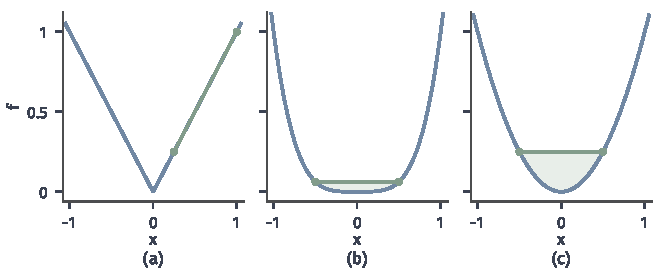
\includegraphics[width=112mm]{figures/05-optimization/01-linear-programming/matplotlib/opt-convexity-gap/figure.pdf}
  \caption{三种弯曲程度下的弦间隔，绿色线段是弦，浅绿区域是间隔。(a)$\lvert x\rvert$在同侧取端点时弦贴着图像，凸但不严格凸。(b)$x^4$严格凸，端点$\pm0.5$的中点处间隔只有$0.0625$。(c)$x^2$是$2$强凸的，同样端点的中点处间隔为$0.25$。}
  \label{fig:opt-convexity-gap}
\end{BookInlineFigure}

\paragraph{目标差控制到解的距离}
强凸性最直接的用途，是把目标值的误差换成位置的误差。

\begin{theorem}[强凸目标的二次增长]
\label{thm:opt-quadratic-growth}
设$\bm{C}$为凸集，$f$在$\bm{C}$上$\mu$强凸，且最优解$\bm{x}^\star$存在。则最优解唯一，并且对所有$\bm{x}\in\bm{C}$，
\begin{equation}
 f(\bm{x})-f^\star\geq\frac{\mu}{2}\lVert\bm{x}-\bm{x}^\star\rVert_2^2.
 \label{eq:opt-quadratic-growth}
\end{equation}
\end{theorem}

\begin{proof}
对$t\in(0,1)$，点$\bm{x}^\star+t(\bm{x}-\bm{x}^\star)$在$\bm{C}$中，目标值不低于$f^\star$。在式~\eqref{eq:opt-strong-convexity}中取$\bm{u}=\bm{x}$，$\bm{v}=\bm{x}^\star$，$\theta=t$，得到
\[
 f^\star\leq tf(\bm{x})+(1-t)f^\star-\frac{\mu}{2}t(1-t)\lVert\bm{x}-\bm{x}^\star\rVert_2^2.
\]

移项后除以$t>0$，得到
\[
 f(\bm{x})-f^\star\geq\frac{\mu}{2}(1-t)\lVert\bm{x}-\bm{x}^\star\rVert_2^2.
\]
令$t\downarrow0$即得式~\eqref{eq:opt-quadratic-growth}。若$\bm{x}$也是最优解，左端为零，迫使$\bm{x}=\bm{x}^\star$。
\end{proof}

证明只用到可行集凸、目标强凸和最优解存在，没有假设解在内部或目标可微。把实例取$\gamma=1$，由式~\eqref{eq:opt-ridge-solution}，$\bm{x}^\star=(2/3,2/3)$，$\mu=1$。取$\bm{x}=\bm{x}^\star+(1,-1)$，两个分量之和不变，所以拟合项不变，目标差全部来自正则项：
\[
 f(\bm{x})-f^\star=\frac12\bigl(\lVert\bm{x}\rVert_2^2-\lVert\bm{x}^\star\rVert_2^2\bigr)=\frac12\cdot2=1.
\]
距离的平方是$2$，式~\eqref{eq:opt-quadratic-growth}的右端也是$1$，在这里取等号，因为位移恰好沿最小特征值的方向。

可行集必须是凸的。$x^2$在$\mathbb{R}$上$2$强凸，但在$C=\{x:\lvert x\rvert\geq1\}$上有两个最小点$\pm1$，两点的目标差为$0$，距离却是$2$。证明中从$\bm{x}^\star$走向$\bm{x}$的线段离开了可行集，那一步就失效了。

表~\ref{tab:opt-convexity-ladder}汇总本节的三级要求及各自多给出的结论。

\begin{BookInlineTable}
  \centering
  \begin{tabular}{@{}lll@{}}
    \toprule
    目标（可行集凸） & 弦下方的间隔 & 结论\\
    \midrule
    凸 & 不小于$0$ & 局部最优即全局最优，解集凸\\
    严格凸 & 大于$0$ & 解至多一个\\
    $\mu$强凸 & 不小于二次量 & 解若存在则唯一，目标差控制距离\\
    \bottomrule
  \end{tabular}
  \caption{沿线段比较的三级要求。每一级都比上一级强，存在性仍需另外保证。}
  \label{tab:opt-convexity-ladder}
\end{BookInlineTable}
